% !TEX program = xelatex
\documentclass[conference]{IEEEtran}
\usepackage{cite}
\usepackage{amsmath,amssymb,amsfonts}
\usepackage{algorithmic}
\usepackage{graphicx}
\usepackage{textcomp}
\usepackage{xcolor}
\usepackage{multicol}
%%% For language switching -- like babel, but for xelatex
\usepackage{polyglossia}
%%% For the awesome fontawesome icons!
\usepackage{fontawesome}
\usepackage{multirow}
\usepackage{makecell} % for more vertical space in cells
\setmainlanguage{english}
\setotherlanguages{hindi,sanskrit} %% or other languages

% define fonts for other languages
\newfontfamily\devanagarifont[Script=Devanagari]{Annapurna SIL}

\def\BibTeX{{\rm B\kern-.05em{\sc i\kern-.025em b}\kern-.08em
    T\kern-.1667em\lower.7ex\hbox{E}\kern-.125emX}}

\makeatletter
\newcommand{\linebreakand}{%
  \end{@IEEEauthorhalign}
  \hfill\mbox{}\par
  \mbox{}\hfill\begin{@IEEEauthorhalign}
}
\makeatother
\usepackage{hyperref}
\title{A Novel Rule-based Recursive Stemming Algorithm for
  Plagiarism Detection in Devanagari Scripts\\
%{\footnotesize \textsuperscript{*}Note: Sub-titles are not captured in Xplore and
%should not be used}
%\thanks{Identify applicable funding agency here. If none, delete this.}
}

\author{\IEEEauthorblockN{Ayush Kumar Shah}
  \IEEEauthorblockA{\textit{Department of Computing and Information Sciences} \\
  \textit{Rochester Institute of Technology} \\
Rochester, NY 14623, USA \\
as1211@rit.edu
}}

\begin{document}

\maketitle

\begin{abstract}
There have been many notable works for detecting plagiarism in the English
texts, but none in the Nepali texts, which uses Devanagari scripts. It is mostly
due to the
involved challenges in the pre-processing of such scripts caused by the lack of
available datasets and the complicated
grammatical rules and structure of the Nepali language. Since
pre-processing texts are vital in performing any Natural Language Processing
(NLP) task, we aim to accomplish this task for Nepali texts. The paper
introduces a rule-based recursive stemming algorithm that effectively handles the
complexities in grammar and the language structure to pre-process Nepali texts.
Furthermore, we use pre-processed texts to develop
a Nepali Plagiarism Detection System using tf-idf feature vector construction
with Cosine similarity measure. The ability to pre-process Nepali texts gives
rise to opportunities to perform various NLP tasks in the Nepali language.
\end{abstract}

\begin{IEEEkeywords}
Plagiarism, Tokens, tf-idf, Affixes, Stemming, Lemmatization
\end{IEEEkeywords}

\section{Introduction}
Plagiarism is one of the increasing crimes brought by increased use of the
internet. It is the act of citing a part or whole document that has been copyrighted without mentioning the author(s) correctly. It is also described as a form of stealing other people's ideas by copying intrinsically
or extrinsically, but still closely resembles the idea of the source document without mentioning its author correctly\cite{r1}. To identify
and deal with this crime, we need to build a system that can detect
plagiarism of any form in texts. A major component of such systems is generating good features from the texts using an appropriate and accurate
stemming algorithm.

There have been many works to address this problem. In 1980, Porter presented a simple algorithm for stemming English language words. This algorithm is the basis
for pre-processing texts until now. Willet \cite{r2} summarises the main features of
the algorithm and highlights its role in modern information retrieval research
and a range of related subject domains. It works well in practice to a
range of languages and has spurred interest in stemming as a topic for research \cite{r2}.  

Over the years many methodologies have been developed to perform automatic detection of 
plagiarism, including tools for natural language text detection such as Turnitin (iParadigms, 2010)
and CopyCatch (CFL software, 2010), and tools for computer programming source code detection such as
MOSS (Aiken, 1994). Various approaches have been developed to deal with both external 
and intrinsic plagiarism in written texts (Lukashenko Graudina \& Grundspenkis, 2007) \cite{r3} 
but mostly in the English language. For instance, the results of applying
several NLP techniques to process a set of suspicious and original documents,
by analyzing strings and the structure of the text, using resources to account for text
relations showed that NLP techniques improve the accuracy of existing approaches 
\cite{r3}. Likewise, Z.Ceska \cite{r4} purposes plagiarism tools based on Singular Value 
Decomposition (SVD) technique like SVDPlag which solves associations among phrases 
contained in the examined documents to infer the mutual similarity of all pairs of the 
documents. Also,  D. Gupta, V. K, and C. K. Singh 
\cite{r5} present a plagiarism detection method, which focuses on detecting 
intelligent plagiarism cases where semantics and linguistic variations play an important role. 
Although these works have contributed significantly to detecting
various forms of plagiarism in English texts, they fail to perform effectively
in scripts of other languages like Devanagari scripts for the Nepali language.
  
This paper aims to overcome the challenges in the task of pre-processing Devanagari scripts. 
Some various complicated grammatical rules and structures need to be considered during the 
pre-processing task. A simple stemming algorithm developed or used in the English language
does not perform well for the Nepali language due to these structural and semantic differences. 
As a result, we aim to develop a novel rule-based recursive stemming algorithm to effectively pre-process the Devanagari scripts and ultimately use it to detect plagiarism between Nepali texts. 

This paper defines several grammatical and syntactic rules to demonstrate the 
rule-based recursive stemming algorithm for Devanagari scripts, followed by the construction
of tf-idf feature vectors on the tokens obtained. Finally, we compute similarity measures 
like Cosine and Jaccard between the resulting vectors to classify the pair of
texts into Plagiarised and Non-Plagiarised classes using a threshold value. We
have obtained an F1-score of 96.55\% on a manually annotated Devanagari
scripts dataset containing 100 pairs of original and suspicious scripts.

\section{Methodology}
\begin{figure}[htbp]
\centering{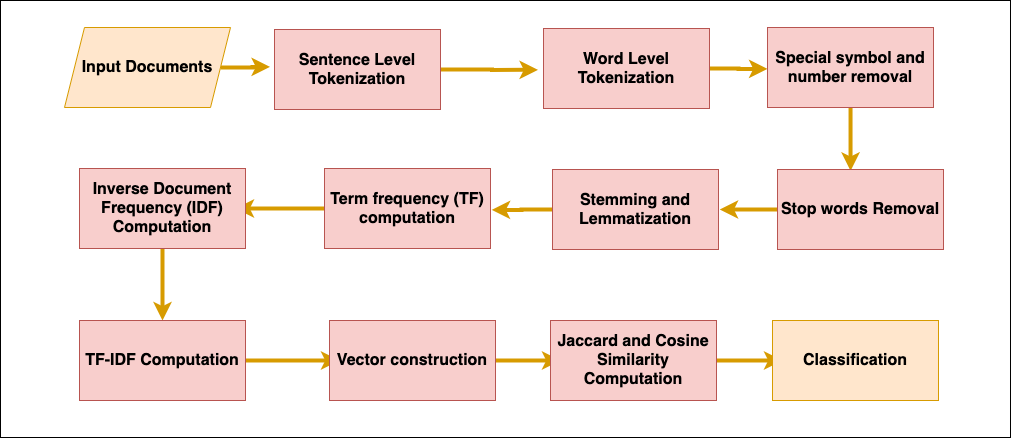
\includegraphics[width=9cm,height=11cm,keepaspectratio]{figures/flow_diagram.png}} 
\caption{Flow diagram for Plagiarism detection showing the major steps} 
\label{flow} 
\end{figure}
% \begin{figure}[htbp]
% \centering
% 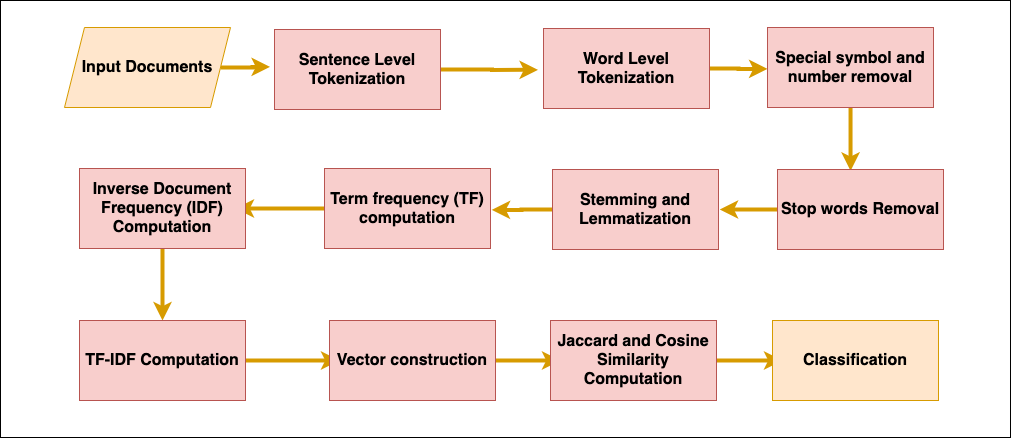
\includegraphics[width=0.525 \textwidth]{figures/flow_diagram.png}
% \caption{Flow diagram for Plagiarism detection showing the major processes
% involved in segmentation and classification}
% \label{fig1}
% \end{figure}

As shown in Figure.~\ref{flow}, there are various operations involved in the
methodology including pre-processing of Devanagari texts using the introduced 
rule-based stemming algorithm, feature vector construction using tf-idf and
finally, similarity computations for the final classifications.

\subsection{Preprocessing of documents}

\begin{enumerate}
\item Sentence tokenization\\
The text in the document is split into sentences, thereby allowing line-by-line
processing in the subsequent sentences. Vertical bars, question marks, and 
exclamation marks are used to break down the text into individual sentences. \\
\\Example:\\\\
\begin{sanskrit}
  "परिश्रम नगरी हुन्छ? परिश्रम सफलताको एक-मात्र बाटो हो। अक्सर जो परिश्रम गर्छ, उही सफल हुन्छ। अब त परिश्रम गर्छौ नि? नगरी कहाँ हुन्छ त!"
\end{sanskrit}\\\\
The following collection of sentences is tokenized into:\\\\
  \begin{sanskrit}
  'परिश्रम नगरी हुन्छ?', 'परिश्रम सफलताको एक-मात्र बाटो हो।', 'अक्सर जो परिश्रम गर्छ, उही सफल हुन्छ।', 'अब त परिश्रम गर्छौ नि?', 'नगरी कहाँ हुन्छ त!'
\end{sanskrit}
\medskip

\item Word tokenization\\
The input sentences are broken down into individual tokens. White space and
comma are used to break down the words. \\
\\Example:\\
\begin{sanskrit}
  
['परिश्रम', 'नगरी', 'हुन्छ?', 'परिश्रम', 'सफलताको', 'एक-मात्र', 'बाटो', 'हो।', 'अक्सर', 'जो', 'परिश्रम', 'गर्छ', 'उही', 'सफल', 'हुन्छ।', 'अब', 'त', 'परिश्रम', 'गर्छौ', 'नि?', 'नगरी', 'कहाँ', 'हुन्छ', 'त!']
\end{sanskrit}
\medskip

\item Special symbol and number removal\\
Special symbols like ,)({}[]?!।"  "":-- and numbers both in English and Nepali are removed from the tokens using regular expressions.
\medskip

\item Stop words removal\\
Stop words are high-frequency words that do not have much influence in the text and are removed to increase the performance.
A list of 592  stop-words like \begin{sanskrit}त्यही, जब, अथवा,\end{sanskrit} were collected, and these words were removed from the list of tokens. 
\medskip

\renewcommand{\labelenumii}{\roman{enumii}}
\item Stemming and Lemmatization\\
Our major contribution is in the stemming and lemmatization algorithm for
Devanagari scripts. Several stemming algorithms are available for the English
language. However, such general stemming algorithms do not perform well for
Devanagari scripts. Unfortunately, there is no algorithm available to stem
Nepali texts which use Devanagari scripts.
Hence, we have developed our algorithm with the help of the 
\href{http://ltk.org.np/}{Language Technical Kendra}.
\medskip

Stemming is a crude heuristic process that chops off the ends of words in the hope of 
achieving root words (morphemes), and often includes the removal of
derivational affixes.
There are two sets of affixes: suffixes and prefixes. The prefixes and suffixes
are stemmed from obtaining a root word.
\medskip

For example, 
In a word \begin{sanskrit} 'सफलताको' 
, 'सफल' \end{sanskrit} is a root and it is combined with the suffix
\begin{sanskrit}‘ता’\end{sanskrit}  and \begin{sanskrit}‘को’\end{sanskrit} and the
resulting form becomes \begin{sanskrit} 'सफलताको'. \end{sanskrit}Some of the prefix
and suffix in the dataset is as follows:
\medskip

We have introduced a rule-based stemming approach, which
agrees with all the grammatical restrictions for stemming the texts in the Nepali language. As a result, the output of the stemming is almost always a
valid root word. It means that the features used to construct vectors are a better representation of the document, while the irrelevant features are removed. A few
prefixes and suffixes are listed below.

Prefix set: \qquad Suffix set:\\
\begin{sanskrit}
न|1\hspace{52pt} यो|17\\
उप|2\hspace{50pt}दा|18\\
महा|3\hspace{48pt}दै|19\\
अ|4\hspace{50pt} ँदै|19\\
सु|5\hspace{54pt}पालिका|20\\
\end{sanskrit}

Here, the number present after the suffix and prefix, delimited by the '|' pipe
sign points to the suffix and prefix rules and used to strip
the affixes.
\medskip

Stemming often results in a word that is only close to the root word which may
not be found in the dictionary. Lemmatization is a more proper process with the
use of vocabulary and morphological analysis of words, normally aiming to remove
inflectional endings only and to return the base or dictionary form of a word, 
which is known as the lemma. These lemmas are obtained by applying the suffix 
and prefix rules repeatedly and using the root word collection for verification.
\medskip

The rules are written in the form:\\
\text{[Rule no][POS][n(sub-rules)][Morpheme][Tag][Ignore]}

\medskip

The number at the beginning indicates rule number, followed by the POS tag, 
number of sub-rules, the morpheme structure, tag, and an N or Y to indicate 
whether to ignore or not to skip the rule for smaller suffixes to be handled.
Below the main rule, are the sub-rules in which the first part is the substring 
to delete from the word and the second part is the substring to insert to the 
word. The dot indicates not to insert any substring \cite{r10}.
\medskip

Some of the rules are:

Prefix rules: \qquad \qquad Suffix rules:\\

\begin{sanskrit}
3 PFX 1 महा महा \qquad \quad 13 SFX 3 छु CHU N\\
महा .\hspace{80pt} ँछ .\\
\phantom{x}\hspace{96pt} न्छु .\\
4 PFX 1 अ NEG \hspace{40pt}छु .\\
अ .\\
\phantom{x}\hspace{96pt}14 SFX 2 छे प N\\
5 PFX 1 सु PTV\hspace{35pt} ँछ .\\
सु .\hspace{88pt} छे .

\phantom{x}\hspace{96pt}15 SFX 2 छौ CHAU N\\
\phantom{x}\hspace{96pt}ँछौ .\\
\phantom{x}\hspace{96pt}छौ .
\end{sanskrit}
\medskip


Example: \begin{sanskrit} खानुभयो खाए खाउ खान्छु to खा  \end{sanskrit}
\medskip

Stemming and Lemmatization Algorithm:

\begin{figure}[htbp]
\centering
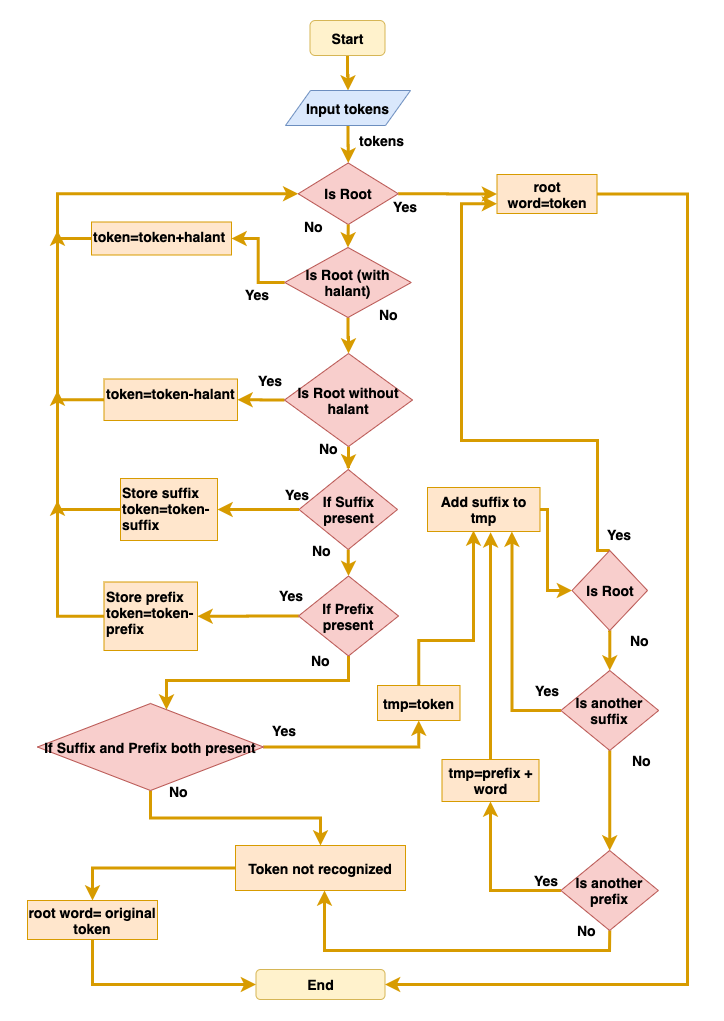
\includegraphics[width=0.45 \textwidth]{figures/stemming.png}
\caption{Detailed Flow diagram for Plagiarism detection including all the
stemming and lemattization steps}
\label{stemming}
\end{figure}

\medskip
Input: A list of pre-processed tokens 

\medskip
Output: A list of lemmas (root words) obtained by striping the affixes using the rules
\medskip

\begin{enumerate}

    \item Check whether the token is lemma or not using the root words and
      alternate root words collections. If root word, return success with the
      token unchanged. If not, go to the next step. \medskip
    
    \item Check whether the token when added to halanta or virama
      \begin{sanskrit}(्)\end{sanskrit} gives a root word or not. If yes, then
      return the corresponding root word as the new token. If not, go to the
      next step.\medskip
    
    \item Check if the token end with halanta or virama
      \begin{sanskrit}(्)\end{sanskrit} and the token without virama gives a root
      word or not. If yes, set the token to the corresponding root word. If not,
      go to the next step.\medskip
    
    \item  Check whether any of the suffixes are present in the token. If yes,
      then strip the suffix using the corresponding rules and set the token as
      the corresponding root word. If not, go to the next step.\medskip
    
    \item Check whether any of the prefixes are present in the token. If yes,
      then strip the prefix using the corresponding rules and set the token as
      the corresponding root word. If not, go to the next step.\medskip
    
    \item If both prefix and suffix are present, recombine the suffix one by one
      and check for lemma verification.\medskip
     
    \item Repeat steps i to vii until root word is found or the token is
      unrecognized.\medskip
    
    \item If the token is unrecognized, return the token without striping else
      return the striped token as the lemma for the token.\medskip
    
\end{enumerate}
\end{enumerate}


\subsection{Feature Vector Construction}
\renewcommand{\labelenumii}{\roman{enumii}}
 \begin{enumerate}
   \item Calculating tf-idf (Term frequency-inverse document frequency)
     \medskip

   Term frequency-inverse document frequency is a statistical measure that
   measures how important a term is relative to a document and a corpus, a
   collection of documents. It is used to construct the vector representation of
   the text documents. Mathematically, the tf-idf of a term is given by the
   equation (\ref{eq1}). 
\begin{equation}tf\textnormal{-}idf(t,d, D) = tf(t,d) \times idf(t, D) \label{eq1}
\end{equation}
   \begin{gather*}
  \text{where},\\
  t=\text{a particular term}, \\
  d=\text{a particular document}, \\
  D=\text{corpus of documents}, \\
  tf(t,d)=\text{term frequency of term t in document d}, \\
  idf(t,D)=\text{inverse document frequency of term t in}\\ \text{a corpus of documents D}, \\
\end{gather*}


So, the tf-idf weight is composed of two terms:
\medskip
   \begin{enumerate}
     \item Normalized Term Frequency (tf)\\
     The term frequency (tf) is the measure of how frequently a term occurs in a
     single document or article. The frequency is normalized by dividing it by
     the total number of terms.
\medskip

A term appearing relatively higher is an important term and has a higher tf
value. Mathematically, the term frequency is given by (\ref{eq2})
\begin{equation}tf(t,d) = \frac{f_d(t)}{\sum_{w\in d}{f_d(w)}} \label{eq2}
\end{equation}
   \begin{gather*}
  \text{where},\\
  f_d(t)=\text{number of term t in document d},\\
  \sum_{w\in d}{f_d(w)} = \text{Total number of terms in}\\ \text{document d}
\end{gather*}\medskip

\item Inverse Document Frequency (idf)\\
     The inverse document frequency (idf) is the measure of how important a term
     is to the entire collection of documents in the corpus. It weighs down the
     effects of terms that occur too frequently while weighs up the effects of
     less frequently occurring terms by inverting the number of documents
     containing the particular term \cite{r6}. We calculate idf for each term
     which is mathematically given by (\ref{eq3})
\begin{equation}idf(t,D) = \ln\left({\frac{|D|}{|\{d\in D : t \in d\}|}}\right) \label{eq3}
\end{equation}
   \begin{gather*}
  \text{where},\\
  |D|=\text{Total number of documents in the corpus},\\
  |\{d\in D : t \in d\}| = \text{Number of documents}\\ \text{\qquad \qquad \quad \quad containing term t}
\end{gather*}
 \end{enumerate}

So, from (\ref{eq1}), (\ref{eq2}), and (\ref{eq3}), we can write the tf-idf as defined in (\ref {eq4})
\begin{equation}
tf\textnormal{-}idf= \frac{f_d(t)}{\sum_{w\in d}{f_d(w)}} \times \ln\left({\frac{|D|}{|\{d\in D : t \in d\}|}}\right) \label {eq4}
\end{equation}

A good example of how idf comes into play is for the word "the." 
We know that just about every document contains "the," so the term 
is not significant, thereby producing a very low IDF \cite{r7}. 

\medskip
    
\item Construction of vector (Vector Space Model)\\
Using the relation in (\ref{eq4}), we construct tf-idf dictionaries for each
term-document pair. Thereupon, we create a matrix that consists of an array of
vectors, where each vector represents a document in the corpus. The vector will
be a list of frequencies for each unique word in the corpus -- the tf-idf value
if the word is in the document, or 0.0 otherwise. The set of documents in the
corpus is then viewed as a set of vectors in a vector space, as shown in Figure.~\ref{vector}.
Each term in the corpus will have its axis \cite{r8}.
\end{enumerate}

\begin{figure}[htbp]
\centering
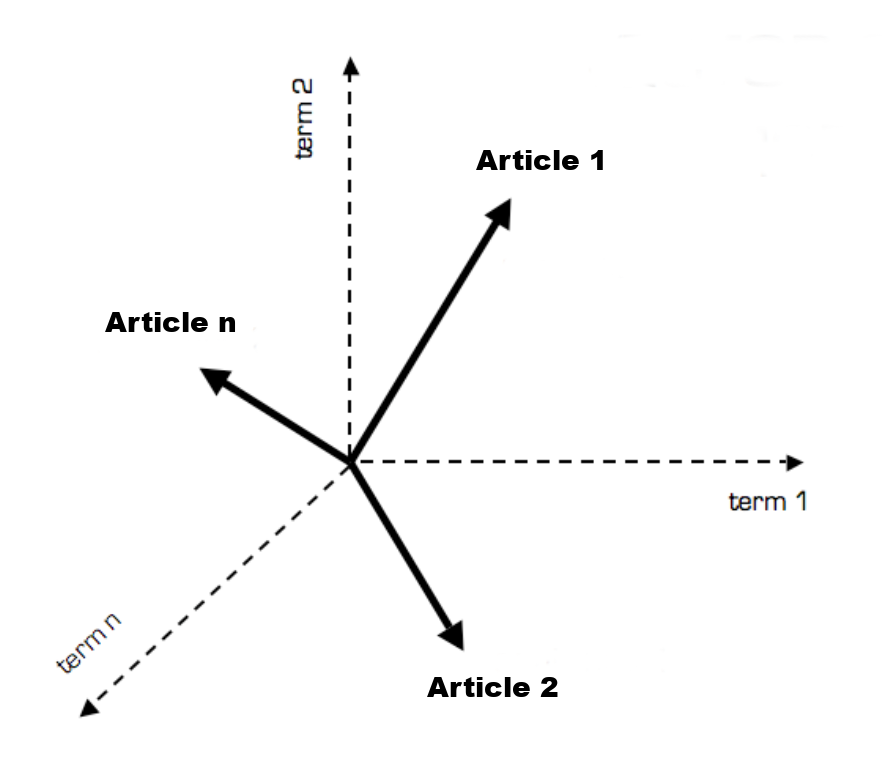
\includegraphics[width=0.4 \textwidth]{figures/vector.png}
\caption{Vector space model.}
\label{vector}
\end{figure}

\subsection{Calculating similarity}\label{AA}
\begin{enumerate}
\item Cosine similarity

It is a metric used to measure the degree of similarity between two
vectors. The vectors' size doesn't affect the similarity value since
the magnitude of the vectors automatically normalizes the value. We use
this metric to compute the similarity between pairs of news articles using the
equivalent tf-idf feature vector representation of the articles. Mathematically,
it measures the cosine of the angle between two vectors projected into a
multi-dimensional space. In this context, the two vectors are arrays containing
each term's tf-idf value in the two documents. 
\medskip

The cosine similarity is
advantageous because even if the two similar documents are far apart by the
Euclidean distance (due to the size of the document), chances are they may still
be oriented closer together. The smaller the angle, the higher, will be the
cosine similarity. When plotted on a multi-dimensional space, where each
dimension corresponds to a word in the document, the cosine similarity captures
the orientation (the angle) of the documents and not the magnitude \cite{r9} as
shown in Figure.~\ref{cosine}. Using the formula given in (\ref{eq5}), we can
find out the cosine similarity between any two documents.

\begin{figure}[htbp]
\centering
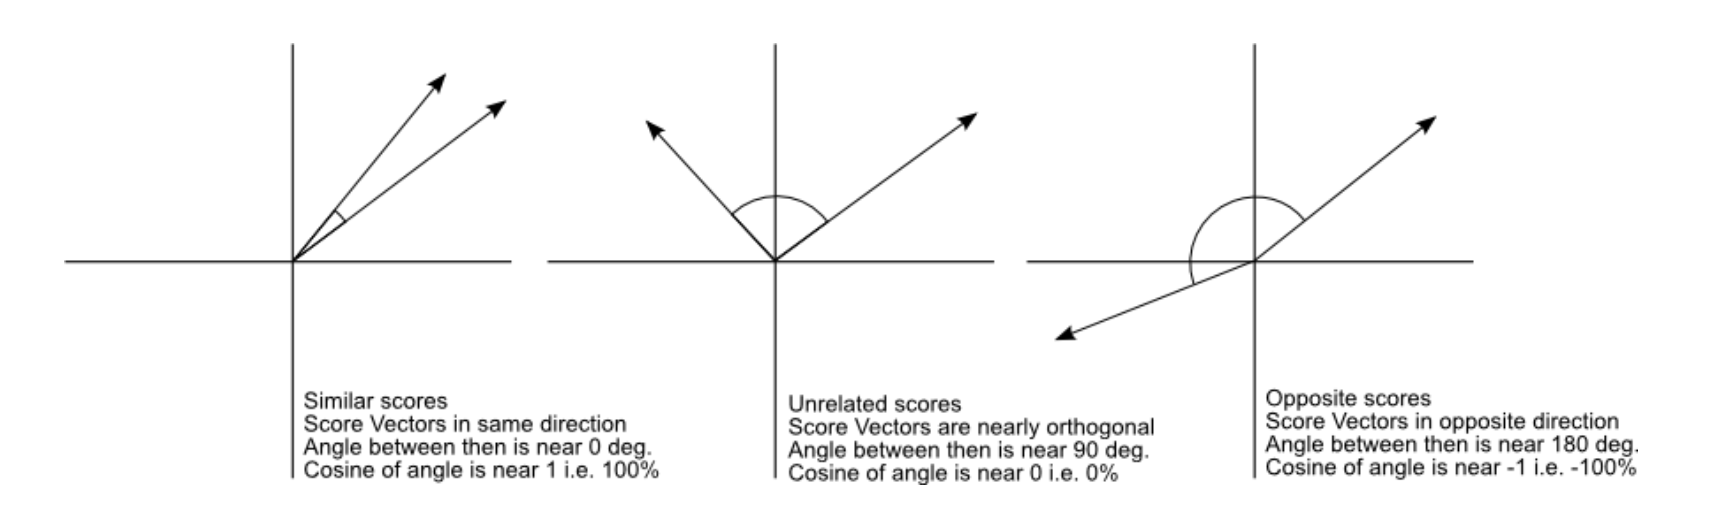
\includegraphics[width=0.5 \textwidth]{figures/cosine.png}
\caption{Cosine similarity visualization}
\label{cosine}
\end{figure}

\begin{equation}
\cos ({\vec a},{\vec b})= {{\vec a} . {\vec b} \over \|{\vec a}\| \|{\vec b}\|} = \frac{ \sum_{i=1}^{n}{{\vec a}_i{\vec b}_i} }{ \sqrt{\sum_{i=1}^{n}{({\vec a}_i)^2}} \sqrt{\sum_{i=1}^{n}{({\vec b}_i)^2}} } \label{eq5}
\end{equation}
 \begin{gather*}
  \text{where},\\
  \vec a \text{ and } \vec b \text{ represents tf-idf vectors of two documents},\\
  n \text{ is the length of the vector or vocabulary size}
\end{gather*}

\medskip

\item Jaccard similarity\\
It is a measure to calculate the similarity between any two documents or terms
or sentences. To calculate the Jaccard similarity, the number of common
attributes is divided by the number of attributes in at least one of
the two objects. Jaccard Coefficient can also be used as a dissimilarity or
distance measure, unlike cosine similarity. If the Jaccard index between two
sets is 1, then the two sets have the same number of elements in the
intersection as the union, and we can show that ${A \cap B=A \cup B}$. So every
element in A and B is in A or B, so ${A = B}$. The Jaccard index can also be
used on strings. We define a set containing the characters in a
string for each string, so the string "cat" becomes {c, a,t}. If we have two strings, "catbird."
and "cat," then the numerator is 3, and the denominator is 7, which gives us a
Jaccard index of 3/7.

\begin{equation}
J(A,B) = \frac{|A\cap B|}{|A\cup B|}=\frac{|A\cap B|}{|A| + |B| -|A\cap B|}\label{eq6}
\end{equation}
\end{enumerate}
\medskip

\section{Results}

One of the major challenges in performing experiments for plagiarism detection
in Nepali texts was the lack of labeled datasets. We collected the following data
from different sources.

\subsection{Corpora}

\begin{enumerate}
\item News articles\\
We collected a pair of 100 Nepali news articles from different online news portals sites.
\medskip

\item Nepali root words\\
A total of 20,641 Nepali root words were collected from \href{http://ltk.org.np}{Language Technical Kendra}.
\medskip

\item Suffixes\\
A total of 135 Nepali suffixes were collected from \href{http://ltk.org.np}{Language Technical Kendra}.
\medskip

\item Prefixes\\
A total of 5 Nepali prefixes were collected from \href{http://ltk.org.np}{Language Technical Kendra}.
\medskip

\item Suffix and prefix rules\\
We wrote the rules for striping the corresponding suffixes and prefixes, respectively, to obtain root words.
\medskip

\item Stop words\\
A total of 592 stop words were collected from multiple online sources.

\end{enumerate}

\subsection{Experiment}

\begin{figure}[h!]
  \centerline{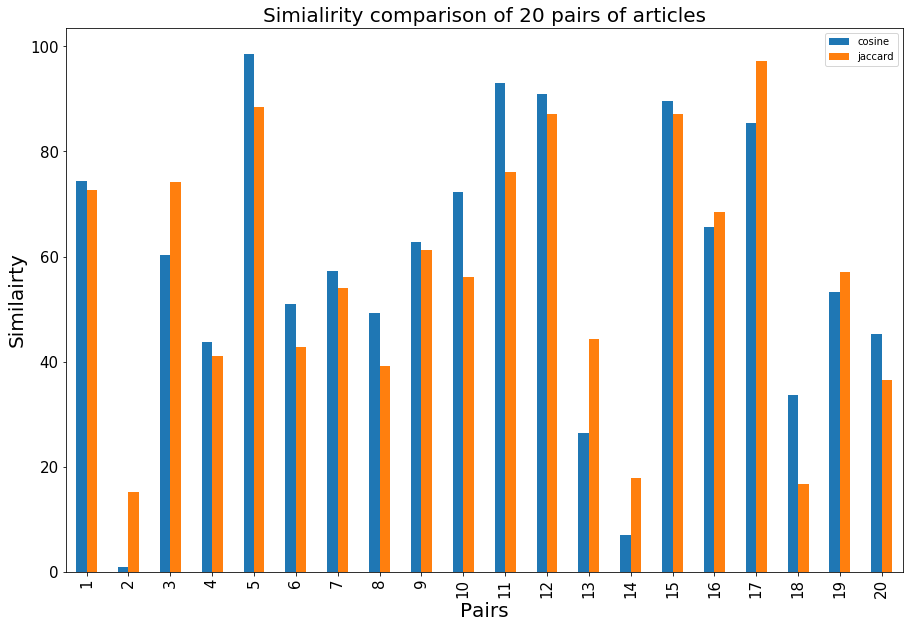
\includegraphics[width=0.4 \textwidth]{figures/similarity.png}}
\caption{Cosine and Jaccard similarity scores comparison for 20 pairs of articles}
\label{similarity}
\end{figure}

For experimentation, we annotated the 100 pairs of news articles
collected from different online news portal sites as plagiarised and
non-plagiarised. Then using our rule-based recursive stemming algorithm, we
performed pre-processing of these articles. The pre-processed texts were then fed
into the feature selection process to construct the tf-idf feature vectors as
per the process explained in the methodology section above. Both Cosine and
Jaccard similarity scores were computed for each pair of articles. The
scores of a sample of a sample of 20 pairs of articles from the corpus 
are shown in Figure.~\ref{similarity}

Comparing the results obtained from Cosine similarity and Jaccard similarity for
all the articles' pairs, we observed that Cosine similarity always yields
better results. Hence, after obtaining the similarity scores, a threshold of
25\% cosine similarity score was used to classify a pair of the article as plagiarised or
non-plagiarised. The confusion matrix obtained in the classification task on 100
pairs of manually annotated articles is shown in Table \ref{conf}. Also, the
results of the evaluation metrics on the same task are shown in Table \ref{eval}.

\begin{table}[htbp]
\caption{Confusion matrix on classification of 100 pairs of manually annotated news articles}
\begin{center}
\begin{tabular}{cc|cc}
\multicolumn{2}{c}{}
&\multicolumn{2}{c}{Predicted} \\
& & Plagiarised & Non-plagiarised\\ 
\cline{2-4}
\multirow{2}{*}{\rotatebox[origin=c]{90}{Actual}}
    & Plagiarised   & 70   & 0                 \\
    & Non-plagiarised  & 5  & 25                \\ 
    \cline{2-4}
    \end{tabular}
\label{conf}
\end{center}
\end{table}

\begin{table}[h!]
\caption{Evaluation Metrics on classification of 100 pairs of manually annotated
news articles}
\begin{center}
\begin{tabular}{|c|c|}
\hline
Accuracy & 95\%\\
Precision & 93.33\%\\
Recall & 100\%\\
F1-Score & 96.55\%\\
\hline
 \end{tabular}
\label{eval}
\end{center}
\end{table}

\section{Conclusion}

This paper introduced a novel stemming algorithm using a set of custom-defined
recursive rules to pre-process   Devanagari
scripts effectively for the Nepali language in order to detect plagiarism with
more precision and recall in Nepali articles. Since a proper pre-processing
method for Devanagari scripts has not been developed yet, this algorithm can be
helpful in various NLP tasks, other than Plagiarism as
well, that need to be performed in such scripts. Most of the NLP
tasks include the pre-processing step before employing the main algorithm or the
required task. Moreover, this algorithm can be extended to other languages as
well by developing similar recursive rules as per the grammatical rules of the
corresponding language. Hence, this paper has a wide range of applications in
the field of NLP. 

The obvious limitation to this approach is the algorithm's non-robust nature 
since the grammatical and syntactic rules required in this algorithm need to be
defined manually, which is dependent on the language completely. Likewise, the
semantic and contextual information in the texts is not considered, which may reduce the performance in a large dataset. Due
to insufficient dataset, the evaluations performed in this paper were done on a
manually annotated dataset, limited in number. Hence, the evaluation may not be a
standard benchmark for comparing the performance.

In the future, we plan to overcome the current limitation by incorporating semantic
and contextual information during the computation of the similarity measures.
One approach may be comparing the similarities of the obtained
tokens' meanings by constructing and using a dictionary instead of the similarities
between the tokens. Thereby, we need to construct a corpus containing Nepali
root words and their corresponding meanings. When similarity is measured at a
semantic level, sentences having different words but giving the same meaning
will get a higher similarity score.

\section*{Acknowledgment}
Our thanks to our supervisor, Associate Professor Bal Krishna Bal,
for assisting and guiding us throughout the project and sincere thanks to 
\href{http://ltk.org.np/}{Language Technical Kendra} for providing us the
required datasets and resources.

\bibliographystyle{IEEEtran} 
\bibliography{references}

\end{document}
